\section{Phase-2 direction: multi-node communication-efficient localization}

The thesis objective is now fixed as obtaining the best fleet localization accuracy with the least UWB communication effort. Two assumptions are treated as given: every node starts from a known initial pose, and every node carries both an IMU and a UWB transceiver and may participate in pairwise ranging.

The primary benchmark will use four symmetric mobile nodes, giving six possible UWB links. Three- and five-node fleets will be retained only as sensitivity cases. Unlike the earlier debugging simulations, ground-truth motion will be defined first through smooth global paths. Ideal velocity, acceleration, yaw, yaw rate, and body-frame IMU signals will then be derived from those paths before sensor noise and bias are added. Pairwise UWB measurements take the form
\begin{equation}
    z_{ij,k}=\|\bm p_{i,k}-\bm p_{j,k}\|_2+\nu_{ij,k},
\end{equation}
so both endpoints are uncertain mobile states.

The new Phase-2 sequence is:
\begin{enumerate}
    \item \textbf{multi-node/full-communication benchmark:} four smooth mobile trajectories, known initial poses, independent IMUs, all six pairwise links available, IMU-only and all-pairs/\SI{10}{Hz} reference cases;
    \item \textbf{uniform rate sweep:} reduce all-pairs UWB rate to establish the basic localization--communication frontier;
    \item \textbf{fixed-budget link selection:} compare round-robin, random, proximity-based, geometry-aware, and information-aware peer/link choices at equal numbers of UWB exchanges;
    \item \textbf{reliability/outage stress:} packet loss, burst outages, and NLOS/outlier processes with an explicit measurement-reliability treatment where required;
    \item \textbf{IMU-quality sensitivity:} determine how the necessary communication budget changes with inertial noise and bias;
    \item \textbf{consolidated frontier:} fleet and worst-node RMSE versus normalized UWB exchanges, later extended to measured energy.
\end{enumerate}

Because the initial pose is known and the new problem is predominantly local/unimodal, a joint fleet EKF is the preferred primary estimator candidate. A short full-communication sanity comparison to the existing PF can be retained, but broad-prior global particle acquisition and AACOPF are no longer the main thesis path.

For \(N\) nodes define the communication ratio
\begin{equation}
    \rho_{\mathrm{comm}}
    =
    \frac{\sum_{k,i<j}a_{ij,k}}
         {K\binom{N}{2}},
\end{equation}
and use fleet position RMSE together with worst-node RMSE as the primary localization metrics. The central Phase-2 result should therefore be an empirical Pareto frontier between localization quality and communication effort.

Phase~3 will use this frontier to develop adaptive policies for \emph{when} to range and \emph{which pair} to range, using uncertainty, geometry/information gain, measurement reliability, and eventually measured energy cost.


\subsection{P2A benchmark result}
The four-node trajectory-first benchmark is now implemented. Across 20 matched seeds, IMU-only propagation gives mean fleet position RMSE \(2.322\pm0.605\)~m, while the maximum-communication reference using all six pairwise UWB links at \SI{10}{Hz} gives \(1.058\pm0.451\)~m. Full communication improves fleet RMSE in all 20 seeds.

The infrastructure-free error decomposition is more important than the aggregate reduction. The fleet-centroid RMSE is essentially unchanged (\SI{1.057}{m} versus \SI{1.056}{m}), while the centered relative-shape RMSE drops from \SI{2.027}{m} to \SI{0.046}{m}. Pairwise UWB therefore removes almost all differential fleet deformation but cannot directly observe a common translation of the complete fleet.

\begin{figure}[htbp]
    \centering
    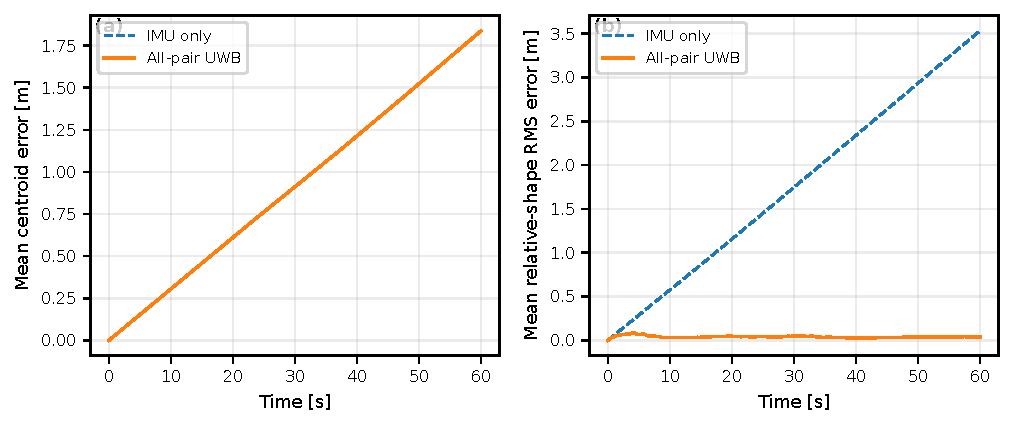
\includegraphics[width=0.94\textwidth]{figures/phase2/p2a_error_decomposition.pdf}
    \caption{P2A error decomposition: pairwise UWB strongly constrains relative fleet geometry while the common global-translation mode remains.}
\end{figure}

\subsection{P2B uniform-rate result}
On the frozen P2A benchmark, the all-six-link rate was swept across \(0,0.5,1,2,5,10\)~Hz with identical sensor draws in each of the 20 matched seeds. These rates cost respectively 0, 180, 360, 720, 1800, and 3600 individual pairwise range exchanges over \SI{60}{s}. Both endpoint conditions reproduce the P2A per-seed results.

Already at \SI{0.5}{Hz}, 180 exchanges (5\% of full communication) lower mean fleet RMSE from the IMU-only \SI{2.322}{m} to \SI{1.064}{m}; the \SI{10}{Hz} reference gives \SI{1.058}{m}. All positive rates improve fleet RMSE against IMU only in all 20 paired runs. This apparent plateau reflects the unobservable common translation: centroid RMSE remains near \SI{1.056}{m}, while relative-shape RMSE continues falling from \SI{0.114}{m} at \SI{0.5}{Hz} to \SI{0.046}{m} at \SI{10}{Hz}. Worst-node RMSE also improves from \SI{1.097}{m} to \SI{1.071}{m} over these rates.

\begin{figure}[htbp]
    \centering
    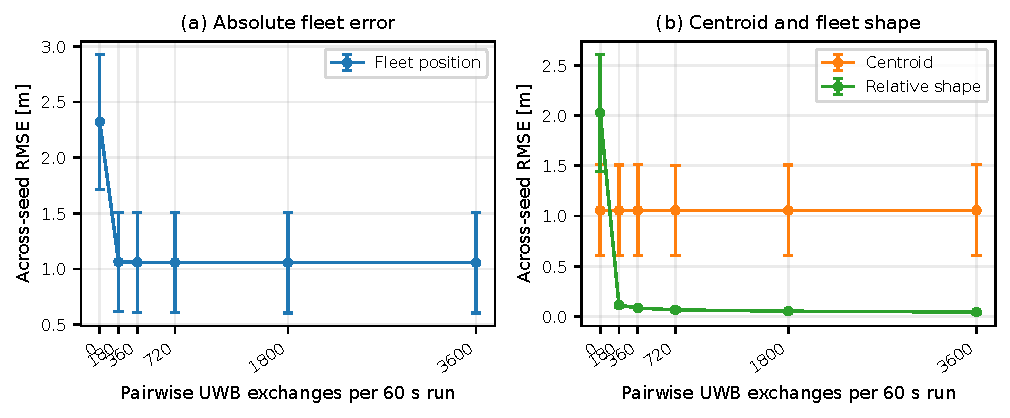
\includegraphics[width=0.94\textwidth]{figures/phase2/p2b_rate_sweep.pdf}
    \caption{P2B uniform-rate reference: mean whole-run error and one across-seed sample standard deviation versus the number of individual pairwise UWB exchanges. Absolute fleet RMSE flattens earlier than relative-shape error.}
\end{figure}

P2C is the next experiment. It will hold these individual-exchange budgets fixed while selecting links and times differently, and compare both absolute fleet and relative-shape accuracy. The P2B curve is an empirical reference for this one scheduling family; lower rates, alternative scheduling policies, and radio energy are not yet measured.

After the infrastructure-free Phase-2 frontier is established, a separate P2G extension will test the value of a global reference. One of the existing four mobile nodes will first supply its true position throughout a matched run, followed by noisy and intermittent position reports. Comparisons will score the same three non-reference nodes and retain matched UWB budgets. This bounds how much a globally localized auxiliary can reduce common drift without changing the symmetric, unanchored main benchmark.
